\section{Evaluation}

\subsection{Practice-as-research}

This prototype has been evaluated with the use of a \textit{practice-as-research} methodology. This evaluative methodology has been chosen for a number of reasons, first of all being the lingering presence of the COVID-19 pandemic which makes in-person user testing very difficult. Furthermore, it offers a unique lens though which to evaluate this prototype. 

Practice-as-research is an extension of the \textit{research through design} methodology presented in \cite{gaver_what_2012}, which is described as the ``the inference of generalisable principles from a set of design artifacts" \citep{martelloni_guitar_2021}.

In \cite{martelloni_guitar_2021}'s work, the authors highlight the following benefits of practice-as-research, which are logical extensions of the benefits of \cite{gaver_what_2012}'s work. 

These benefits include the affordance of \textit{pre-paradigmatic research}, which is beneficial because the artefact can be evaluated outside of an established set of rules and standards, and this diversity of analysis, Gaver argues, is beneficial to the scientific and research effort.     

Secondly, \cite{martelloni_guitar_2021} highlight a second benefit, put forth by \cite{carey_reection_2016}. This is shown by the concept of the \textit{bricolage} approach to research. This means that ``there is quick feedback on the design, as evaluation and prototyping are brought forward in parallel by the same person or the same group of people". This may mean tighter, and more effective circles of design iteration.

To perform this practice-as-research, the author has used the prototype to compose a new song. This presents an ecologically valid situation for the prototype (in a music studio, in the hands of a guitarist), as well as the benefits listed above.

The piece is available to listen to \href{https://drive.google.com/file/d/1AR7ZPBJgG3uJql0nhqeoFNKMg3zadOTz/view?usp=sharing}{\textbf{here}}. 

The piece was composed using Ableton Live 11 for Microsoft Windows 10. This was chosen since the software has native MPE support \citep{ableton_mpe_2021}. It would still be possible to complete the composition in another DAW which does not have native MPE support, but this would require creating 16 instances of each software instrument, each with a unique MIDI channel, to take advantage of the prototype's MPE functionality. It would also make editing software instrument parameters extremely cumbersome since each of the 16 instances would need to be manually updated individually. Using a DAW with native MPE support avoid this. 

In the following sections we will be exploring a critical analysis of the process in the creation of the author's composition, with respect to the role that the prototype played, and how it changed the way the track was composed. 

\subsubsection{Sound design}
In the composition of the piece, the first thing that was a barrier to creativity was the size of the palette of sounds available that takes advantage of the MPE features of the prototype. The author had developed a preset for Ableton's \textit{Wavetable} synthesizer for debugging and development of the prototype, but beyond this, there did not exist a large palette of sounds to draw from. 

To solve this, composition was stopped, and the author performed a sound design session, creating a set of 16 sounds which take advantage of both the aftertouch and pitch bend abilities of the controller. This step made the process of composition much more straightforward, and less frustrating. 

Sounds that employ the full feature-set of this prototype are typically legato, that map aftertouch to amplitude and brightness (usually by mapping to a low-pass filter cutoff frequency). One typically expects the pitch bend range to be roughly -2 to +2 semitones, which is typical, however there are more experimental sounds that fully employ the pitch bend feature of the prototype, mapping from -24 to +24 semitones. 

\subsubsection{Playing the parts}
The actual prototype is overall quite expressive, and perceivably offers a high degree of fine control over aftertouch and pitch bend features. However, since it was a novel instrument to the author, much of the `muscle memory' that had built up as a traditional guitarist was not as directly translatable as was expected. This meant that performing some parts of the composition such as the lead line, had to be performed a number of times to record a performance that was free of mistakes. 

\subsubsection{Composition}
Overall, the process of composition was subjectively very removed from using a typical non-MPE MIDI controller.

% Why it was easier?
% Why was it more difficult?
% Why it was more inspiring?
In the following ways, the prototype was more creatively inspiring than a non-MPE controller.
 
With the appropriate MPE enabled software instruments, the individual note expression made for a novel experience in comparison to the author's previous experience inputting MIDI into a DAW. This novelty perceivably was in itself a component of the success of the instrument, but this does not speak to it's specific nature that much. 

Speaking directly as a function of the individual note expression, this was able to create much more idiosyncratic synthesizer recordings, that would be incredibly tedious to manually program with a mouse. The lead line of the given composition is a prime example of this. Within the four bar loop of the main theme, each note event is completely unique with respect to its duration and aftertouch envelope. This has the subjective effect of creating a more `organic' or `human' feeling in the music, which represents a successful implementation of the MPE techniques.

% Why it was less inspiring?
However, the composition process was made more cumbersome with the use of the prototype, insofar as the author's muscle memory had not completely entrained with the nature of the instrument yet, and this nature of being unable to convert intention to reality was at times frustrating. This can be understood as a natural function of it being a new instrument, but one of the aims of this prototype is to be able to more directly translate previously available muscle memory to the MIDI domain. This offers a direction for improvement in future iterations of the design.

Though the novelty was very inspiring, this layer of frustration prohibited some level of creativity.

% Why it was less practical? 
In comparison to the desktop, keyboard style MIDI controllers, guitar-like MIDI controllers, MPE enabled or otherwise, may be less suitable for studio applications than previously thought. 

In a practical sense, having a keyboard on the desk in front of the musician or producer is a `natural', and well established studio practice. However, the practicalities of balancing a guitar on one's lap, while leaning over to try and start recording, or editing MIDI, after a few hours in the studio is more creatively draining than simply accessing a MIDI controller that is at rest on the desktop. 

Though this is perhaps a minor observation, if our goal is to optimise the creative potential for users, this is a problem worth examining. 

% Talk about how it's harder to express your ideas, because it requires you to be able to play the instrument well, and you're not perfect at playing the instrument well yet, which made it more frustrating than necessary. 

% What are some of it's overall successes? 
Subjectively, the author believes that the addition of authentic human expression in the composition is successful. This links to studies such as \cite{witek_syncopation_2014}, which discuss the effect of groove and imperfect timing on the increased enjoyment of music, at least in particular styles. 

It was also interesting that, since editing many notes of MPE material in post-production is laborious and cumbersome, this invited performing more takes of the performance to get a satisfactory recording. This practice supports musicianship in favour of over-editing, which can often make for a more authentic musical experience. 

% !!!!!!!!!!!!!!!!!! Can we do a COGNITIVE WALK THROUGH???????? !!!!!

% WHAT KIND OF ERROR IS THE STRING MISMATCH ERROR????? NORMAN!

% HOW DO WE STACK UP AGAINST OUR GOAL OF MARTELLONI'S DIGITAL PHONBIA ETC???

% How does it contrast to using a typical MIDI keyboard?


% % What would you do to fix the issues you raised above?
% KEY ISSUES:
% - difficult to hold in sat down in the studio
% - not matchign muscle memoery from tradiditonal guitar
% - not currently having open string triggers, which does not support traditional guitar-style strumming or playing. 
% - creatively draining in the long term (of a session).
% - needs wires tidying up. 
% - wants haptic feedback on the neck, insofar as you can 'feel' the strings like you can on a normal guitar. This would probably help with the transition, but this may conflict with the expression of the strings. Maybe just put haptic feedback on the string boundaries. 

% KEY BENEFITS:
% - musically expressive and more authentic performances. 
% - fun!
% - supports creativity in the short term
% - pitch bend/vibrato is successful! 

% \subsubsection{Listening and reflection}

% % Okay, so what sort of things do we need to do? Dunno! Um. 

% % Listening. 

% % On listening, it's pretty, uh more human, but you can hear more of the mistakes. 

% % Though I'm not an expert in playing it, it's pretty cool. You need more time to get the shit right. 

% % You need to spend more time practicing with it, which is annoying, but could reap big rewards.

% \subsubsection{Aspects to develop in the next design iteration}


\subsection{Heuristic Evaluation}

To further extend the evaluation of the prototype, we can conduct a heuristic evaluation. Heuristic evaluation is a method for identifying the usability problems in a user interface design \citep{nielsen_usability_1994, nielsen_heuristic_1990}. Since our prototype is indeed a type of user interface, this evaluative process can add some value to this study. 

Heuristic evaluation consists of generally a number of `expert' user interface designers who will assess the system (our prototype) to a number of `heuristics', these are outlined briefly in Appendix \ref{appendix:heuristics}.

By walking step by step through these heuristics we highlight a number of successes of the design, but also elements which could be improved. By highlighting these areas for improvement, we hope to contribute to the better understanding of prototyping this type of NIME for future researchers and practitioners. 

It is noted that not all of the points analysed here relate directly to the MPE functionality of the prototype, but the frustrations of points raised will cumulatively impact the prototype's ability to support creativity in general, and creating a device that is supportive of creativity is one of the goals of this study.

% MENTION THAT YOU'RE AWARE THAT MAYBE THIS IS A WONKY WAY TO EVALUATE NIME. MAYBE YOU SHOULD ALSO EVALUATE WITH RESPECT TO SOME MORE NIMEY LITERATURE?

Furthermore, the author notes the work of \cite{rodger_what_2020}, noting that traditional HCI evaluation of NIME is not necessarily the most effective. \cite{rodger_what_2020} argue that since instruments are more completely described with reference to their context. The affordances of any one instrument interact with and constrain other affordances and processes of its interconnected systems, for example connected DAWs and digital synthesizers. The authors summarise the issue neatly with the following quotation:

\begin{quote}
    ``Instruments can do and mean many different things that are not easily delimited by a predetermined functional teleology, and this is affected by their evolution among other instruments and musical practices." \\ 
    \hspace*{\fill} \textit{\cite{rodger_what_2020}}
\end{quote}

Traditional HCI evaluation makes the implicit assumption that precision, control and accuracy are valued \cite{rodger_what_2020}, but many subjectively successful NIME do not conform to this assumption \cite{gurevich_expression_2007}. However, this instrument \textit{does} happen to value control and precision, and since it is a new type of instrument, the following heuristic evaluation offers a broad-strokes analysis of the benefits and shortcomings of the design as it stands. 

\subsubsection{Visibility of system status}
Since the system only has a limited set of states, either `on' or `off', it is tempting to imagine that there is not need for system feedback beyond a simple power LED. However, this is only a prototype, and as the feature-set grows to incorporate strumming modes, and other input modes, users should be able to know that the system is in fact in the right `mode'. This will help avoid mode errors, which can be very frustrating for a user. One might imagine a user on stage with this digital instrument, about to perform a solo, but their instrument not properly signify which mode it was in, and result in an undesired output, and unhappy concert-goers. 

Currently, while the prototype is indeed a prototype and bound to wired studio use, the power indicator on the Bela board is likely sufficient, but as the features grow, this will change and more sophisticated signifiers of mode will be required.



\subsubsection{Match between system and the real world}
Since this is a new system, which does not behave the same way as a `traditional' guitar, we say there is an unnatural mapping between our prototype and the traditional guitar. In this sense there is arguably not a great match between the system and the `real world' of the traditional guitar, which some users may find jarring.

We might consider two solutions to this. Either, the prototype should support traditional guitar style playing, so that users can use the system in a way which matches up with their expectations, or it is somehow able to make it clear to the users what \textit{is} possible with the prototype and what is \textit{not}. This could be done with forcing functions by having definitively no place to strum, and thus prohibit this behaviour, for example. 

However the latter is not conducive to this study's goal of creating a system which is conducive to creativity. A system that aims to foster creativity should have affordances for self-expression that support users in as many ways as possible. 

\subsubsection{User control and freedom}
This heuristic is effectively a question of whether the device supports undoing mistakes, or cancelling unwanted tasks. 

This heuristic is not so applicable to our prototype in it's current state just like heuristic \textit{1)}. However this is something to be aware of in future iterations. If a user accidentally changes mode, it should take one \textit{easily identifiable} `click' or button press to get back to where they were. 

\subsubsection{Consistency and standards}
This prototype implements MIDI, which is a standardized digital protocol. This prototype should, and broadly does, apply this standard. However, this is necessary but not sufficient. Most MIDI instruments exhibit a `plug-and-play' functionality, which means that as soon as they are plugged into the computer, they immediately begin to work. This is a convention that the prototype does follow by using the Bela `Run project on boot' functionality as can be seen in Figure \ref{fig:runonboot}. 

\begin{figure}[h]
    \centering
    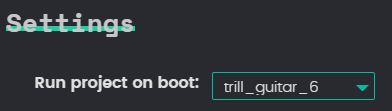
\includegraphics[scale=0.8]{Images/run on boot.png}
    \caption{The Bela IDE's `Run project on boot' functionality.}
    \label{fig:runonboot}
\end{figure}

However, the Bela ambiguously identifies its MIDI port as `Midi function', as can be see in Figure \ref{fig:midifunction}. It is a typical practice for MIDI devices to identify themselves with a helpful name such as "AugGuitar Prototype V1.0" for example.

\begin{figure}[h]
    \centering
    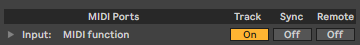
\includegraphics[scale=0.8]{Images/midi function.png}
    \caption{The Bela MIDI device appearing with as `MIDI Function' in the MIDI ports list of Ableton Live 10. }
    \label{fig:midifunction}
\end{figure}

This is a type of \textit{external} inconsistency \citep{nielsen_heuristic_1990}, and is likely to confuse users on the first time using it, which may impede their creativity. 

\subsubsection{Error prevention}

As highlighted in the section above, the lack of visual and haptic (for example emulating the physical sensation of strings across the sensors) feedback as to the position of string centres does not support error prevention particularly well. 

It is not very forgiving of accidental incorrect finger placement, and only permits users who already have a muscle memory of the position of the strings to work without error. Despite being the developer of the prototype, even the author does not possess this ability. 

The addition of haptic feedback (e.g. dummy strings across the sensors) would also be more supportive of visually impaired users, which would be beneficial. 

On the other hand, the prototype's pitch bend functionality is more successful in this sense. Where the prototype does not bend the note, regardless of initial touch location and the addition of the $\alpha$ exponent in expression \ref{eq:pitchbend} helps in the reduction of unwanted pitch bends. This should help make the experience less frustrating, and ultimately more creatively supportive. 

\subsubsection{Recognition rather than recall}
There are few things to have to remember about the current design with respect to it's usability. Insofar as there are no deep menus to traverse. Thus, this heuristic is less applicable to the prototype than some of the others. 

\subsubsection{Flexibility and efficiency of use}
Under heuristic \textit{2)} we touched on a point about some users that will want, or expect, the prototype to function like a traditional guitar. In this way, the prototype is not flexible, since it only supports one style of playing. To amend this, a greater number of playing styles could be supported, which would increase the flexibility and usability of the prototype. 

\subsubsection{Aesthetic and minimal design}
Currently the prototype is very minimal indeed, and certainly does not show superfluous information to the user. It might be argued that the vestigial volume and tone knobs, and pick up selector tack against this heuristic, but they naturally would not continue into later iterations of the design since they serve no functional purpose in the system.

\subsubsection{Help users recognize, diagnose and recover from errors}
Currently, the prototype offers implicit feedback to slips where the wrong note is pushed, because the wrong note will sound. However this point is somewhat of a triviality.

As the prototype develops, it should offer more sophisticated feedback to general troubleshooting issues such as drivers failing to load, etc. However, issues like this are not the concern of this prototype. 

% IT ALSO COULD BE INTERESTING TO SHOW AN APP THAT SHOWS THE TOUCH LOCATIONS IN REAL TIME JUST LIKE IN THE BELA DEMOS. 

\subsubsection{Help and documentation}
This heuristic is also less applicable to this prototype. The interface being a guitar shape is reasonably self-evident, but as the feature-set grows supporting documentation about driver installation should be created as required. 
 % GAHHH NOT REALLY APPLICAABLE! ANYWAY TIME FOR A BREAKKKKKKKKKKK. 



% However as the system is reasonably complex, and has a number of sensors which may be incorrectly connected or otherwise faulty, we might imagine a use being confused at the lack of feedback if something 







